\documentclass[sans,mathserif]{beamer}
%handout,notes=show

%\usepackage{pgfpages}
%\pgfpagesuselayout{8 on 1}[a4paper,border shrink=5mm]

\usetheme{default}
\usepackage{fp}
\usepackage[thicklines]{cancel}
\usepackage{tikz}
\usepackage{multirow}
\usepackage{amsmath}
\usepackage{ifthen}
\usepackage{animate}
\usepackage{setspace}
\usepackage{forloop}
\usepackage{tikz}

%\usepackage{concmath}
%\usepackage{pxfonts}
%\usepackage{eulervm}
%\usepackage{mathpazo}
%\renewcommand\mathfamilydefault{\rmdefault}

%\usefonttheme{professionalfonts}
%\setmathfont{}
%\setsansfont{Palatino}
\usetikzlibrary{arrows,backgrounds,positioning,fit,chains,shapes,calc}

%\usepackage{handoutWithNotes}
%\pgfpagesuselayout{4 on 1 with notes}[a4paper,border shrink=5mm]

\setbeamertemplate{navigation symbols}{}

\title{Hashdist -- Yet Another Desperate Attempt at Fixing Scientific Software Distribution}
\author{Dag Sverre Seljebotn (Simula Innovation AS)\\Ond\v{r}ej \v{C}ert\'{i}k (U. of Texas, TACC)\\Chris Kees (US Army ERDC)}
%\institute{Department of Mathematics \\ University of Oslo}
\date{ITA, February 27, 2013}

\newcommand{\V}{\vskip1em}

\setbeamersize{sidebar width left=0cm, sidebar width right=0cm}
\setbeamersize{text margin left=.8cm, text margin right=.8cm}

\defbeamertemplate{note page}{infolines}
{%
  \vskip3em
%  \setstretch{1.8}
  \Large
  \rmfamily
  \insertnote
}
\setbeamertemplate{note page}[infolines]

\renewcommand{\CancelColor}{\color{red}}

\begin{document}


\begin{frame}
  \titlepage

  \begin{center} {\tt http://github.com/hashdist}
  \end{center}
~

{\footnotesize

Dag Sverre's work for Simula Innovation is funded by a grant from the \\
International Research Office, US Army Engineer Research and Development Center
(BAA contract W911NF-12-1-0604)
}

\end{frame}


\begin{frame}
  \frametitle{Rest of the world in 2013...}

  \begin{itemize}
    \item<+-> Debian/RedHat
    \item<+-> App stores
    \item<+-> Web apps
    \item<+-> Libraries for business \& web: Smaller and smaller
      \begin{itemize}
        \item<+-> Treshold for sharing something smaller
        \item<+-> a) git and GitHub, b) Google and Twitter et al.
      \end{itemize}
  \end{itemize}
\end{frame}

\begin{frame}
  \frametitle{Scientific code}
  \begin{itemize}
  \item<+-> Dependencies are bad: Hard to build, move between clusters
  \item<+-> Dependencies are good: Can build on works of others
  \item<+-> Often happens: ``Large frameworks'' bundling things together
    \begin{itemize}
    \item<+-> PETSc and Trilinos for solving PDEs
    \item<+-> Smaller example: Fortran HEALPix incl. Gaussian RNG
      \begin{itemize}
      \item What if you want inverse-Gamma RNG?
      \end{itemize}
    \item<+-> As soon as you want to push boundaries there's a lot of dirty work ahead
    \end{itemize}
  \end{itemize}
\end{frame}

\begin{frame}[fragile]
  \frametitle{What makes scientific codes so special?}

  \begin{itemize}
    \item<+-> No root access
    \item<+-> Sometimes you {\bf need} the very latest version
    \item<+-> Fortran/C++ instead of C/Java/.NET
    \item<+-> Intersection of ``need speed'' and ``do not pay dedicated application sysadmins''
  \end{itemize}
\end{frame}

\begin{frame}[fragile]
  \frametitle{Combinatorial explosion}

\uncover<+->{
\small {\tt

/cluster/software/VERSIONS/hdf5-1.6.1/lib/libhdf5.so \\
/cluster/software/VERSIONS/hdf5-1.6.1\_intel/lib/libhdf5.so \\
/cluster/software/VERSIONS/hdf5-1.6.1\_pgi/lib/libhdf5.so \\
/cluster/software/VERSIONS/hdf5-1.8.9/lib/libhdf5.so \\
/cluster/software/VERSIONS/hdf5-1.8.9\_intel/lib/libhdf5.so \\
/cluster/software/VERSIONS/hdf5-1.8.9\_pgi/lib/libhdf5.so \\
}}

~

\uncover<+->{
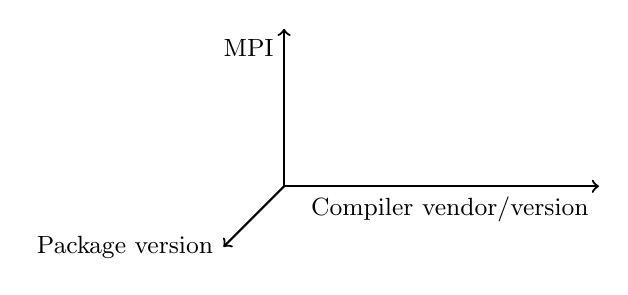
\begin{tikzpicture}[scale=2]
    \draw[thick,->,black] (0,0,0) -- (2,0,0) node[anchor=north east]{\small Compiler vendor/version};
    \draw[thick,->] (0,0,0) -- (0,1,0) node[anchor=north east]{\small MPI};
    \draw[thick,->] (0,0,0) -- (0,0,1) node[anchor=east]{\small Package version};
\end{tikzpicture}

~

$\times$ LAPACK $\times$ FFT library $\times$ IDL/Python version...
}

\end{frame}



\begin{frame}
  \frametitle{Established options elsewhere}

  \begin{itemize}
  \item<+-> Debian/Ubuntu/RedHat/Gentoo
    \begin{itemize}
    \item<+-> Need root
    \item<+-> Deals poorly with combinatorial explosion
    \end{itemize}
  \item<+-> MacPorts, Fink
    \begin{itemize}
    \item<+-> Mac only
    \item<+-> Deals ``not good enough'' with combinatorial explosion
    \end{itemize}
  \item<+-> HPC environment modules
    \begin{itemize}
    \item<+-> The sysadmins hate them
    \item<+-> The users need newer/their own libraries
    \end{itemize}
  \end{itemize}

\end{frame}

\begin{frame}
  \frametitle{Current solutions}
  \begin{itemize}
  \item<+-> Build yourself from source
    \begin{itemize}
    \item<+-> {\tt ./configure -\,{}-prefix=\$HOME/local; make; make install}
    \item<+-> {\tt export LD\_LIBRARY\_PATH=\textasciitilde{}sigurdkn/local/lib}
    \item<+-> Fragile, duplication of work...
    \end{itemize}
  \item<+-> Aha! Make a script to build from source...
    \begin{itemize}
    \item Simula: dorsal
    \item 5 different within DoD (incl. python-hpcmp)
    \item Sage
    \item Lots of others (``everybody'' does it)
    \end{itemize}
  \item<+-> Easy to do oneself $\Rightarrow$ difficult for one to get
    momentum
  \item<+-> The details are different for everybody
  \end{itemize}

\end{frame}


\begin{frame}
  \frametitle{Curation}
  
  \begin{itemize}
  \item<+-> Debian, RedHat, cluster sysadmins, dorsal is all about curated software stacks
  \item<+-> Perhaps you want 60\% curated, 20\% bleeding edge or manually tweaked, 20\% your own code...
  \end{itemize}
\end{frame}


\begin{frame}
  \begin{itemize}
  \item<+-> Others have failed, we're trying yet again
  \item<+-> Need to have new ideas
  \end{itemize}
\end{frame}

\begin{frame}
  \begin{center}
    {\Large Theory}
  \end{center}
\end{frame}



\begin{frame}
  \frametitle{Hash function}
  {\Large
\[ h(k) : \mathbb{N} \to \mathbf{H} \]
}
\end{frame}


\begin{frame}
  \frametitle{Digression -- $O(1)$ hash table table lookups}


\uncover<+->{
  \begin{center}
    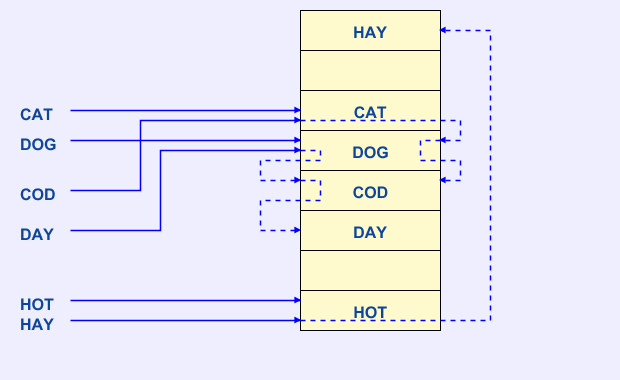
\includegraphics[width=.8\textwidth]{hashtable.png}
  \end{center}
}

\uncover<+->{
If you know contents up front: Create {\em perfect} $h$
}

~

\uncover<+->{
{$h$ should be very fast; don't care so much about properties}

{\small Image: Hopgood (1968), Computer Bulletin}
}
\end{frame}

\begin{frame}
  \frametitle{Cryptographic/secure hashing}

  \begin{itemize}
  \item<+-> Large key size (160, 256, or 512 bits)
    \begin{itemize}
    \item NIST standards: SHA-1, SHA-2 (224, 256, 384, 512 bits), SHA-3
    \end{itemize}
  \item<+-> Mathematical research topic to make $h$ such that no
    information about input is revealed
  \end{itemize}

~

\uncover<+->{
\small
\only<3>{$h$({\tt 'The dark fox'}) = $h$({\tt 546865206461726b20666f78} hex) \\
\quad  = {\tt b6589fc6ab0dc82cf12099d1c2d40ab994e8410c} hex}
\only<4>{$h$({\tt 'The dark fog'}) = $h$({\tt 546865206461726b20666f67} hex) \\
\quad  = {\tt da4b9237bacccdf19c0760cab7aec4a8359010b0} hex}%
}


\end{frame}

\begin{frame}
  \frametitle{Example 1: Store passwords}

Use the one-way nature

\end{frame}

\begin{frame}
  \frametitle{Example 2: git}
~

\only<1>{

\tt
\$ (cd code/hashdist/.git/objects; find)
./59/5a2f8e3890d0ece24514f3e32ae874f1f03ac2 \\
./2f/780151688e1f122a5b9072d42009c80c36140c \\
./2f/4b2eef40b51bc2d46027d1864653b37dd05f8f \\
./2f/237d74e3f81f498212629ac0b96bedac4b0b36 \\
./2f/dff799c54fed6fe96a91e1d5f1593996228ebc \\
./2f/27bd4efa5f8521fb98eb82181a67aae97b7f1a \\
./2f/3fedf882f1b28905199961356f4e00281ddf76 \\
}
\only<2->{
  \begin{center}
    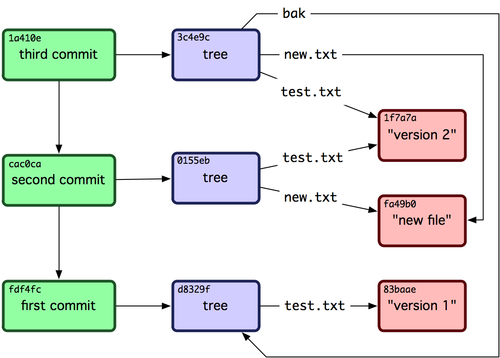
\includegraphics[width=.8\textwidth]{githashes.png}
  \end{center}
}
\end{frame}

\begin{frame}
  \frametitle{Why hashes?}
  \begin{itemize}
  \item<+-> Incremental database IDs don't work for distributed systems
  \item<+-> Random ID's would work...
    \begin{itemize}
    \item E.g., UUID like {\tt 550e8400-e29b-41d4-a716-446655440000}
    \end{itemize}
  \item<+-> ...but a hash simultaneously verifies the content!
  \end{itemize}

\end{frame}

\begin{frame}
  \begin{center}
    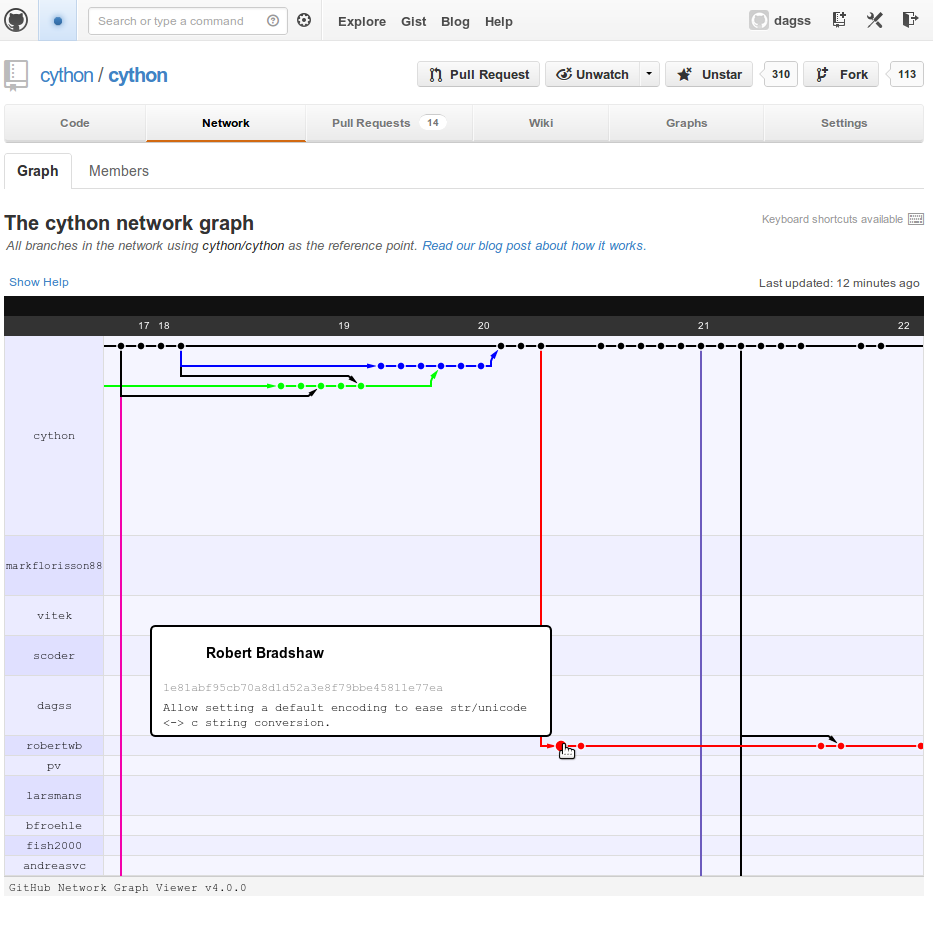
\includegraphics[width=.9\textwidth]{github-screendump.png}
  \end{center}
\end{frame}

\begin{frame}
  \frametitle{Chances of collision...}
\uncover<+->{
Types of attack (assume $k=160$):

\begin{itemize}
  \item<+-> Preimage attack: Chance $2^{-160} \sim 10^{-50}$
  \item<+-> Accidental collision: May happen in a collection of $2^{80} \sim 10^{25}$
    keys due to ``birthday paradox''
    \begin{itemize}
    \item 6.5 billion programmers...
    \item ...each produce one Linux kernel history every second...
    \item ...and push to one enourmous Git repsitory...
    \item ...then after 5 years there's a 50\% chance of collision
    \end{itemize}
  \item<+-> Brute-force SHA-1 still needs only $2^{60}$ operations due to weaknesses
in SHA-1
\begin{itemize}
\item \$2.5M today, \$50K after 2020.
\end{itemize}
\end{itemize}
}
\end{frame}

\begin{frame}
  \begin{center}
    {\LARGE Hashdist}
  \end{center}
\end{frame}

\begin{frame}[fragile]
  \frametitle{Hash-based installation}

  \begin{itemize}
  \item<+-> Linux laptop:
{\small
\begin{semiverbatim}
/usr/lib/libhdf5.so
\end{semiverbatim}
}
  \item<+-> HPC environment modules:
{\small
\begin{semiverbatim}
/cluster/software/VERSIONS/hdf5-1.6.1/lib/libhdf5.so
/cluster/software/VERSIONS/hdf5-1.6.1_intel/lib/libhdf5.so
/cluster/software/VERSIONS/hdf5-1.6.1_pgi/lib/libhdf5.so
/cluster/software/VERSIONS/hdf5-1.8.9/lib/libhdf5.so
/cluster/software/VERSIONS/hdf5-1.8.9_intel/lib/libhdf5.so
/cluster/software/VERSIONS/hdf5-1.8.9_pgi/lib/libhdf5.so
\end{semiverbatim}

  \begin{itemize}
  \item<+-> Even {\tt
      h5py-hdf5\_1.8.9\_pgi-python2.7-numpy1.6.3\_abel\_debug}
    incomplete
  \item<+-> Abel is new and small; US Army clusters have 20-30 versions of every package.
  \end{itemize}
}
    \item<+-> Hashdist:
{\small 
\begin{semiverbatim}
~/.hit/opt/hdf5/{\color{red}efn3}/lib/libhdf5.so
~/.hit/opt/hdf5/{\color{red}i7ni}/lib/libhdf5.so
~/.hit/opt/hdf5/{\color{red}qgpd}/lib/libhdf5.so
\end{semiverbatim}
}
{\footnotesize (really {\tt hdf5/efn3i7ni7lbtik4frlb5wcnqgpdmi3ql})}
  \end{itemize}
\end{frame}

\begin{frame}[fragile]
  \frametitle{Step 1: Hash the build}
\uncover<+->{{\bf Internal protocol!}}
{\footnotesize
\begin{semiverbatim}
\{
   "name": "hdf5",
   "import" : [\{ "id" : "gcc/apyicmxgafb564zz7rwhwvon7padvxdx"\},
               \{ "id" : "unix/v-1"\},
               \{ "id" : "zlib/wbg27phinbgwjg4nasb4xzf3ypo72otn"\}],
   "sources" : [\{ "key" : "tar.bz2:7jxgwn5xs5xnvsdaomvypridodr35or2"\}],
   "cmd": ["sh", "$in0"],
   "inputs": [
       {"text": [
            ["./configure --prefix=$\{ARTIFACT\} --with-pic \\\\"],
            ["    --with-zlib=$ZLIB\only<3->{{\color{red} CFLAGS='-O0 -g'}}"],
            ["make"],
            ["make", "install"]
        ]}]
\}
\end{semiverbatim}
}

~

\uncover<+->{Hash to create key $\rightarrow$
\only<2>{{\tt \footnotesize hdf5/u4vsabroylchvmwoxf5mdpxidd4lnrwl}}%
\only<3->{{\color{red} \tt \footnotesize hdf5/fjczhadqtyx6jlbnvzlthrzsex7wz7xb}}
}

\end{frame}

\begin{frame}[fragile]
  \frametitle{Step 2: Every build installs to separate location}
Same as with the ``module load`` system:

\begin{semiverbatim}
\$ echo opt/*/*
opt/hdf5/avnj opt/hdf5/a5df opt/hdf5/a4sf opt/python/arxd
opt/python/rvdo opt/readline/6vvu  opt/readline/v7fw
opt/zlib/fh7n  opt/zlib/i7yr ...

\$ ls opt/zlib/fh7n/lib
libz.a  libz.so  libz.so.1  libz.so.1.2.5  pkgconfig

\$ ls opt/hdf5/avnj/lib
libhdf5.a  libhdf5.so  libhdf5.so.7  libhdf5.so.7.0.4
\end{semiverbatim}
\end{frame}

\begin{frame}[fragile]
  \frametitle{Step 2: Every build installs to separate location}
Unlike ``module load`` we don't need LD\_LIBRARY\_PATH:
\begin{semiverbatim}
\$ ldd opt/hdf5/avnj/lib/libhdf5.so
  linux-vdso.so.1 =>  (0x00007fff54b7a000)
  libpthread.so.0 => /lib/x86_64-linux-gnu/libpthread.so.0
  libm.so.6 => /lib/x86_64-linux-gnu/libm.so.6
  libz.so.1 => ${ORIGIN}/../../../zlib/fh7n/libz.so.1
  libc.so.6 => /lib/x86_64-linux-gnu/libc.so.6
  /lib64/ld-linux-x86-64.so.2
\end{semiverbatim}
\end{frame}


\begin{frame}[fragile]
\frametitle{Step 3: Make a profile with links}
\begin{semiverbatim}
\$ ls -la opt/profile/ldhn/bin
h5dump -> ../../../hdf5/avnj/bin/h5dump
h5import -> ../../../hdf5/avnj/bin/h5import
h5ls -> ../../../hdf5/avnj/bin/h5ls
...
\end{semiverbatim}
\end{frame}


\begin{frame}[fragile]
\frametitle{Branchable software stack}

\begin{itemize}
\item<+->
\begin{semiverbatim}
\textasciitilde{}/mystack \$ ls
default.yml sources.yml build.yml abel-cluster.yml
\end{semiverbatim}

\item<+->
\begin{semiverbatim}
\textasciitilde{}/mystack \$ hit update # takes some time
\textasciitilde{}/mystack \$ ~/local/bin/python --version
Python 2.7.2
\end{semiverbatim}
\item<+->
\begin{semiverbatim}
\textasciitilde{}/mystack \$ hit update # instant
\end{semiverbatim}

\item<+->
\begin{semiverbatim}
\textasciitilde{}/mystack \$ git fetch from-someone-else
\textasciitilde{}/mystack \$ git checkout someone-elses-branch
\textasciitilde{}/mystack \$ hit update # pause for extra builds
\textasciitilde{}/mystack \$ ~/local/bin/python --version
Python 2.7.3
\end{semiverbatim}

\item<+->
\begin{semiverbatim}
\textasciitilde{}/mystack \$ git checkout paper-from-2010
\textasciitilde{}/mystack \$ hit update # instant
\textasciitilde{}/mystack \$ ~/local/bin/python --version
Python 2.6.3
\end{semiverbatim}
\end{itemize}
\end{frame}


\begin{frame}[fragile]
  \frametitle{Consequences of hash-based installation}
  \begin{enumerate}
  \item<+-> More dimensions! Even \\
{\footnotesize
{\tt .../h5py-hdf5\_1.8.9\_pgi-python2.7-numpy1.6.3\_debug\_ubuntu12.10}
}
is not exhaustive; ``{\tt h5py/5ffg...}'' caters for everything

  \item<+-> For free: Atomic upgrades
\begin{semiverbatim}
\$ hit upgrade
# ...then power shuts down, but you're good
\end{semiverbatim}

  \item<+-> Much easier: Uninstall (mark\&sweep rather than file tracking)

  \item<+-> Jump around in software history (or between branches) in seconds!


  \end{enumerate}

~

\uncover<+->{
  \begin{center}
    {\bf Sophisticated features with simple implementation}
  \end{center}
~

Prior art: Eelco Dolstra's PhD thesis/the Nix project
}
\end{frame}


\begin{frame}
  \frametitle{Status}
  \begin{itemize}
  \item<+-> Hashdist-as-a-library up and running, lacks user interface
    \begin{itemize}
    \item UI = how to describe a ``package''
    \end{itemize}
  \item<+-> Starting to use it for ``python-hpcmp'' (US Army PETSc + Python distribution)
    \begin{itemize}
    \item Shell scripts and {\tt Makefile}s replaced with Hashdist to provide more features
    \end{itemize}
  \item<+-> Up next: Need to provide one (out of many) UI
  \end{itemize}
\end{frame}


\begin{frame}
  \frametitle{Ideas for autumn}

  \begin{itemize}
  \item<+-> Specifying the entire software stack in minute detail is bothersome
  \item<+-> Want a constraint solver
    \begin{itemize}
    \item A[version$\ge$2] needs B[version$\ge$1.2]
    \item B[version$\ge$1.1] needs LAPACK=intel-mkl
    \item Given constraints, solve for LAPACK-type and A-version, B-version
    \end{itemize}
  \item<+-> Debian does constraint solving between packages
    \begin{itemize}
    \item But we have $\prod_{i\in\{\text{MPI},\text{compiler},...\}} n_i$ possible ``packages''
    \end{itemize}
  \item<+-> We want to do constraint solving on input variables to the build
  \item<+-> Objective function: Miminimize build time or maximize package freshness?
  \item<+-> NP-complete problem (``SAT solving''), need heuristics, e.g.:
    \begin{itemize}
    \item Integer linear programming
    \item Belief propagation (from Bayesian network theory)
    \end{itemize}
  \end{itemize}

\end{frame}

\begin{frame}
  \frametitle{Why bother?}

  \begin{itemize}
  \item<+-> Leaving build input variables free (e.g., LAPACK)
    allows ``re-seating'' a software stack description from one system
    to another
  \item<+-> Small step towards the ``reproducible paper''
  \end{itemize}
\end{frame}



\begin{frame}
  \begin{center}
    {\Large The end}
  \end{center}
\end{frame}

\begin{frame}
  \frametitle{The tradeoff: Builds must be ``functional''}
  \begin{itemize}
  \item<+-> All dependencies and all of the environment must be
    taken into account when describing the build
  \item<+-> More hassle, but very good for reproducibility
  \end{itemize}
~
\uncover<+->{Some help:}
~
\begin{itemize}
\item<+-> Integrate with host system (Debian, environment modules,
  ``generic'') to specify dependencies on package on host system
\item<+-> ``hdist-jail'' can issue warnings if a build process
  accesses files it shouldn't (or hide them)
\end{itemize}
\end{frame}

\begin{frame}[fragile]
\frametitle{User-facing software stack definitions}
Declarative approach (because you can git it and share it):

{\small

\begin{semiverbatim}
include:
  - sources # pull in ./sources.yml
  - build
  - when cluster == "abel":
    - abel-overrides
profiles:
  - name: "default"
    configuration:
      lapack_type: "openblas"
      cluster: "hexagon"
    select:
      - project: "hdf5"
        version: 1.8.2\only<2>{{\color{red} to 1.8.5 # with integer linear programming}}
      - project: "h5py"
        ...
\end{semiverbatim}
}
\end{frame}

\begin{frame}[fragile]
\frametitle{For stack developers: DSL focused on overrides}

Manage the combinatorial explosion without creating
packages for {\tt hdf5\_intel\_mpich}, {\tt hdf5\_gcc\_openmpi}, ...:
{

\begin{semiverbatim}
rules:
  ...
  CFLAGS: ["-g", "-O\$optlevel"]
  when recipe == "configure-make-install":
    optlevel: 2
  when project == "hdf5":
    recipe: "configure-make-install"
    when version == 1.5.2:
      optlevel: 0
    build_deps:
      - project: "zlib"
        version: 1.2.5 to 1.2.7
  ...
\end{semiverbatim}
}
\end{frame}

\begin{frame}[fragile]
  \frametitle{Temporary internal representation in Hashdist}

{\small
\begin{semiverbatim}
dict(
 package='hdf5',
 version='1.8.10',
 recipe='configure-make-install',
 downloads=['http://www.hdfgroup.org/ftp/HDF5/current/'
            'src/hdf5-1.8.10.tar.bz2'],
 sources=['tar.bz2:7jxgwn5xs5xnvsdaomvypridodr35or2'],
 configure=['--prefix=${ARTIFACT}', '--with-pic'],
 CFLAGS=['-O2'],
 jail='warn',
 build_deps=[zlib, unix, gcc]
)
\end{semiverbatim}
}
\end{frame}


\begin{frame}[fragile]
  \frametitle{For Hashdist developers}

Feed it through a Python pipeline:
{\footnotesize

\begin{semiverbatim}
@pipeline.add\_recipe('configure-make-install')
def configure\_make\_install\_recipe(ctx, cfg, build):
    build['build']['script'].extend([
        ["LDFLAGS=$(hdist", "build-ldflags", ")"],
        ["CFLAGS=$(hdist", "build-cflags", ")"],
        ["CFLAGS+= " + " ".join(cfg.CFLAGS)],
        ['./configure'] + cfg.configure,
        ['make'],
        ['make', 'install']
        ])
\end{semiverbatim}
}

\end{frame}

\begin{frame}[fragile]
  \frametitle{Generated, read by Hashdist developers while debugging}

{\footnotesize

\begin{semiverbatim}
\{ "import" : [\{ "id" : "gcc/apyicmxgafb564zz7rwhwvon7padvxdx"\},
               \{ "id" : "virtual:unix"\},
               \{ "id" : "zlib/wbg27phinbgwjg4nasb4xzf3ypo72otn"\}],
   "sources" : [\{ "key" : "tar.bz2:7jxgwn5xs5xnvsdaomvypridodr35or2"]\},
   "script" : [
        ["LDFLAGS=$(hdist", "build-ldflags", ")"],
        ["CFLAGS=$(hdist", "build-cflags", ")"],
        ["CFLAGS+= -O2"],
        ["./configure", "--prefix=$\{ARTIFACT\}"]
        ["make"],
        ["make", "install"]]
\}
\end{semiverbatim}
}

\end{frame}


\end{document}